\makeatletter
\renewcommand{\fnum@figure}{Figure \thefigure}
\makeatother

\chapter{Experiments} \label{chap:experiments}

To identify whether the Dirichlet Multinomial Regression method proposed can provide richer and more valuable information than single-output or deterministic methods can alone, we ran experiments on the data obtained from the ACFR's Sirius AUV and Schmidt's Falkor. The main machine learning algorithms' performance which we tested were Gaussian Process Classification, and Dirichlet Multinomial Regression. In this section, the experiments were designed to display the benefits of a Gaussian Process Classifier's probabilistic output, as well as the label distributions of a Dirichlet Multinomial Regressor.

\section{Training Data}
To perform our experiments, bathymetry data and images of Scott Reef Central were used (the reef in the centre of \autoref{fig:scottreefaerial}). The bathymetry data was collected using Eric Schmidt's Falkor, a ship dedicated to marine research, and the (over 700GB) of images corresponding to all the bathymetry data was collected by The University of Sydney's Australian Centre for Field Robotic's Sirius Autonomous Underwater Vehicle (AUV). The training set provided already had labels assigned, which was a result of previous efforts using Variational Dirichlet Processes that performed the unsupervised clustering \citep{steinberg11}. On close inspection, the UTM coordinates in the training set do not correspond to the original data available from \cite{squidle} - this was because the exact point of retrieval for the bathymetry and image weren't exact matches. To account for this, labels corresponding to bathymetry points were in fact taken from the closest images, rather than exact longitude/latitude or UTM matches, although the UTM coordinates in the training data itself remains as the original.

\todo{(describe the specific features - depth, aspect, rugosity, etc.)}

\begin{figure}
    \includegraphics{scott_reef_aerial.jpg}
    \caption{Aerial shot of Scott Reef from \cite{NASA:SRI}}
    \label{fig:scottreefaerial}
\end{figure}


\section{Data Preprocessing}

\subsection{Downsampling the Data}
As the purpose of using Dirichlet Multinomial Regression was to be able to model the distribution of habitat label occurrences over an area, we downsampled the combined 2011+2015 dataset which was at a siginficantly higher resolution than the 2009 dataset \todo{(calculate how much perhaps)}. Two methods of downsampling in particular were tested. The first coarser approach involved simply taking the space in which the data was collected and placing grids of fixed size over them as in \cref{fig:gridsplit}, binning all points falling within each grid into a single datapoint. Each of these data points contained multiple points from the original dataset with their own counts for each of the possible labels, so the downsampled points simply took the sum of all the label counts in each fixed grid. 

The second summed label counts in the same way, but clusters were instead formed by first calculating the full dendrogram on the 16502 entries in the training data, and forming groups such that none had more than 5 of the original points within them, and the sub-clusters (at each level of the dendrogram) were no more than a 21 metres away from one another. As can be seen in \cref{fig:dendrogram}, the gradual merging into the single supercluster was quite consistent, indicating the original datapoints were mostly evenly distributed.

For a fair comparison between Gaussian process classification and dirichlet multinomial regression, the downsampled data was used to train the GPs as well - although this seems like an unnecessary handicap to the GP, it is more appropriate considering that one of the aims here is to demonstrate what sort of information can be gained from a DM vs. a GP, given the same \textit{raw} data.

\begin{figure}[H]
    \includegraphics[scale=0.6]{training_map_fixedgrid.pdf}
    \caption{Fixed-sized grids placed over training data}
    \label{fig:gridsplit}
\end{figure} 
\begin{figure}[H]
    \centering
    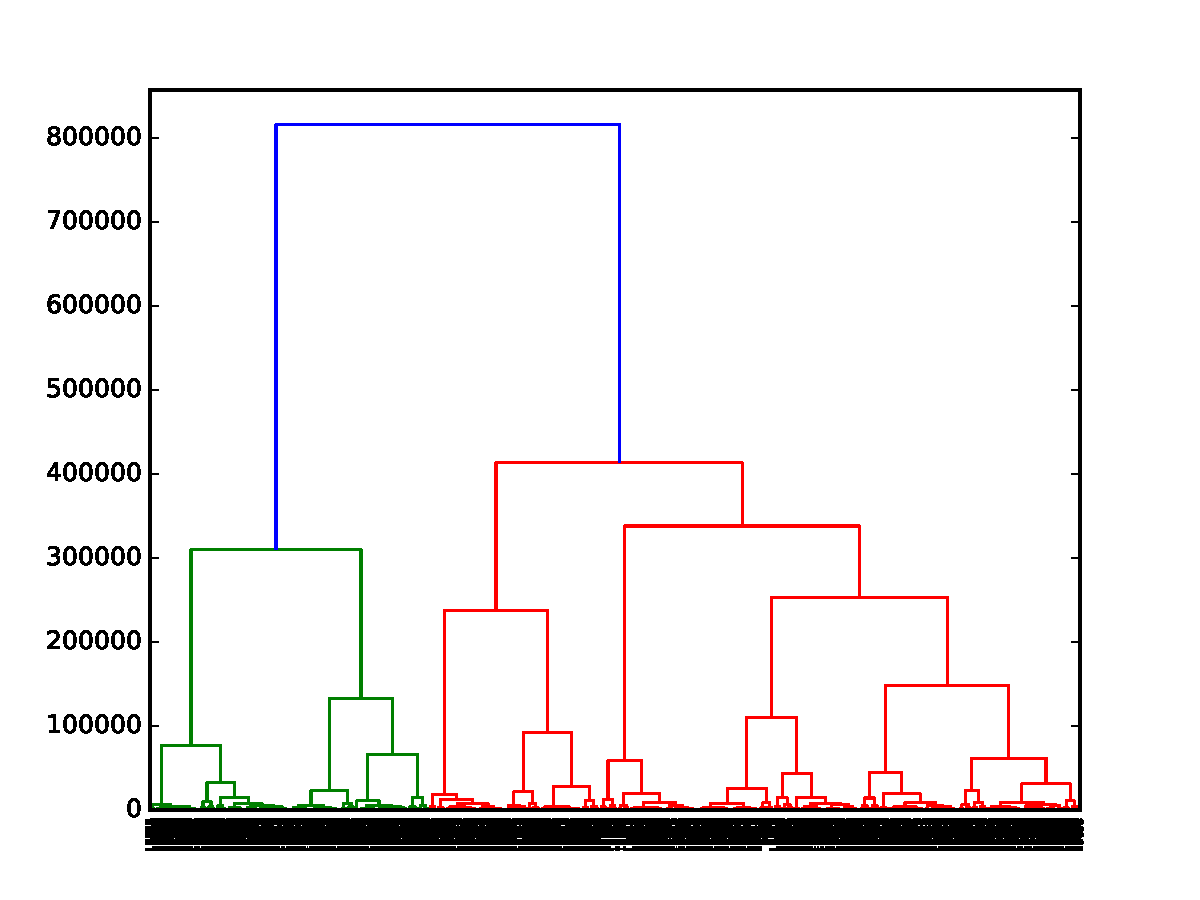
\includegraphics[scale=0.6]{dendrogram.pdf}
    \caption{Dendrogram of training data}
    \label{fig:dendrogram}
\end{figure}

\subsection{Simplifying labels}
Another step that was considered during experiments was the aggregation of habitat labels. The original training data contained 24 separate labels determined through an automated clustering procedure using Dirichlet Processes. Because of the uneven distribution of these labels (\autoref{fig:singlelabeldistr} and \autoref{fig:multilabeldistr}), with the occurrence of some too insignificant for any machine learning algorithms to pick up, they were simplified in collaboration with ecological experts, who manually identified which of the 24 labels were in fact of the same class - for example, 5 separate classes of coral may have been indistinguishable to the average person, and were hence grouped into a single label. This allowed the near-non-occurring labels to be grouped together with more commonly occurring ones, whilst also allowing a different level of granularity in training models/forming predictions that could be used if only an approximation equivalent to observable human differences of an area's benthic map were required. Moreover, due to the unsupervised nature of the labeling, certain clusters were notably \textit{inconsistent} with the rest, for example when sea cucumbers became the identifying feature of one of the 24 labels.

\todo{label mappings - give the labels for the simplified classes, e.g. coral, etc.}

\begin{tabular}{|c| c|}
    \hline
    simplified & original \\\hline
    0 & 1, 2, 18, 20, 21, 23, 24 \\
    1 & 3, 5, 10, 16, 17, 19, 22\\
    2 & 13, 14, 15 \\
    3 & 4, 6, 7, 8, 9, 11, 12 \\
    \hline
\end{tabular}

\todo{put some images here from both original and simplified classes. don't use squidle's downloader, visit server directory and d/l from there directly, 100x+ faster}

\begin{figure}[H]
    \begin{minipage}{.49\linewidth}
        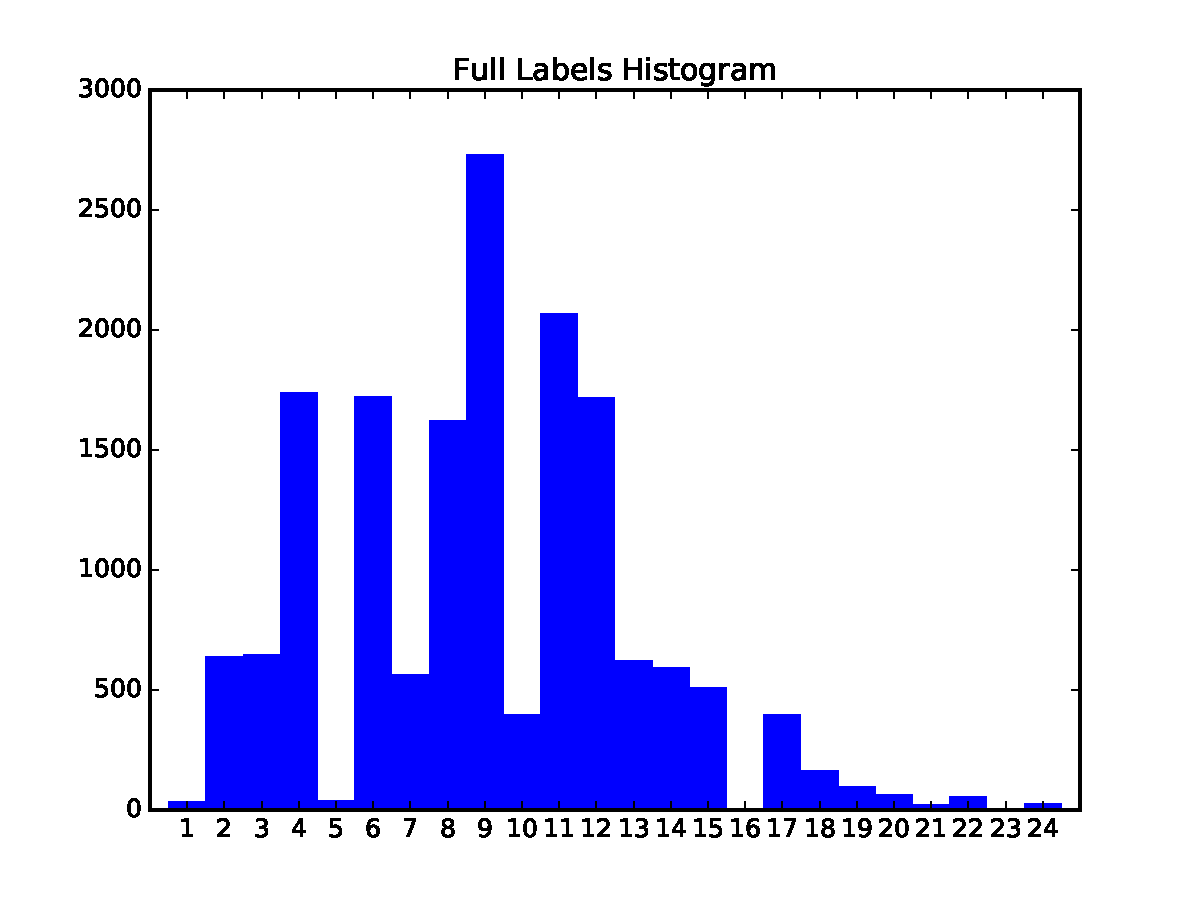
\includegraphics[width=\linewidth]{hist_full_labels.pdf}
        \caption{Distribution of labels in original dataset}
        \label{fig:singlelabeldistr}
    \end{minipage}
    \hfill
    \begin{minipage}{.49\linewidth}
        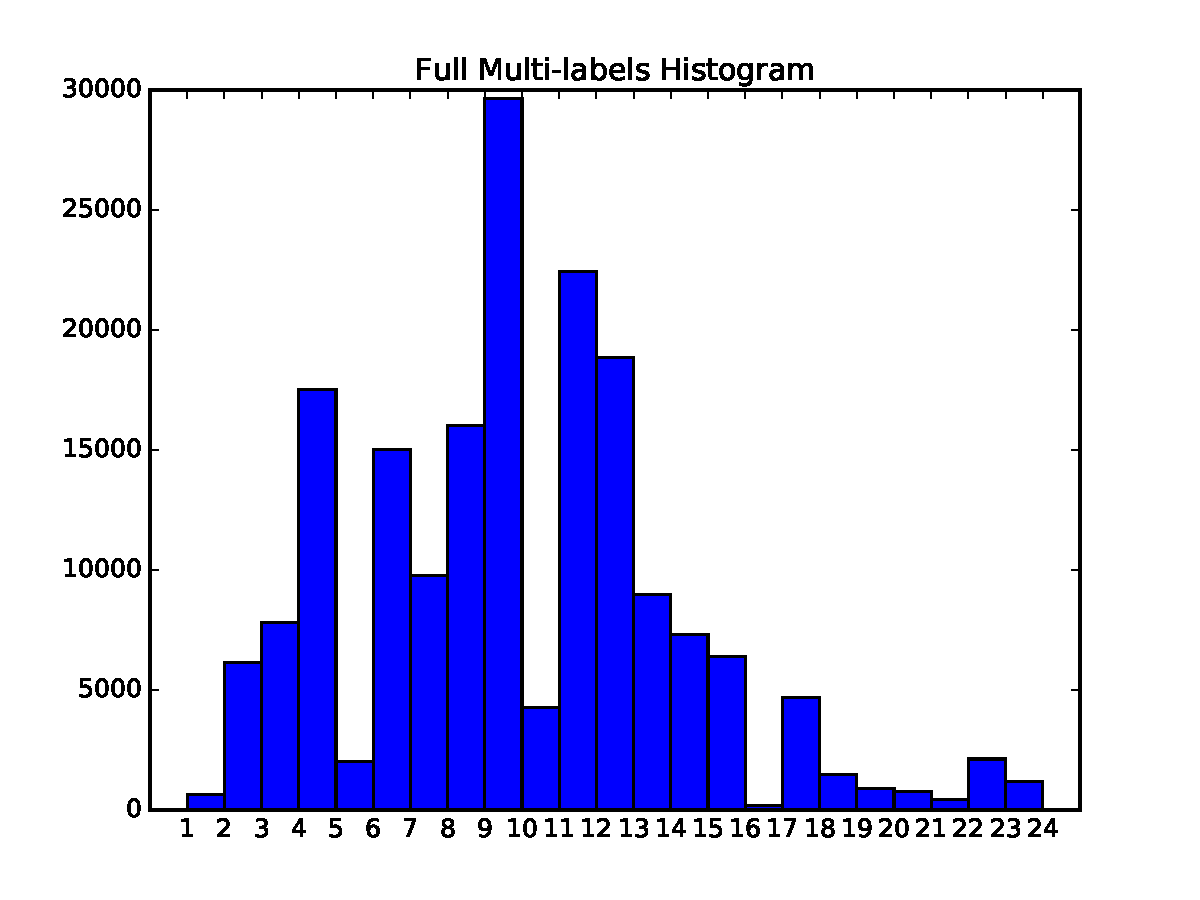
\includegraphics[width=\linewidth]{hist_full_multi_labels.pdf}
        \caption{Distribution of labels in multi-label outputs}
        \label{fig:multilabeldistr}
    \end{minipage}
\end{figure}

\begin{figure}[H]
    \begin{minipage}{.49\linewidth}
        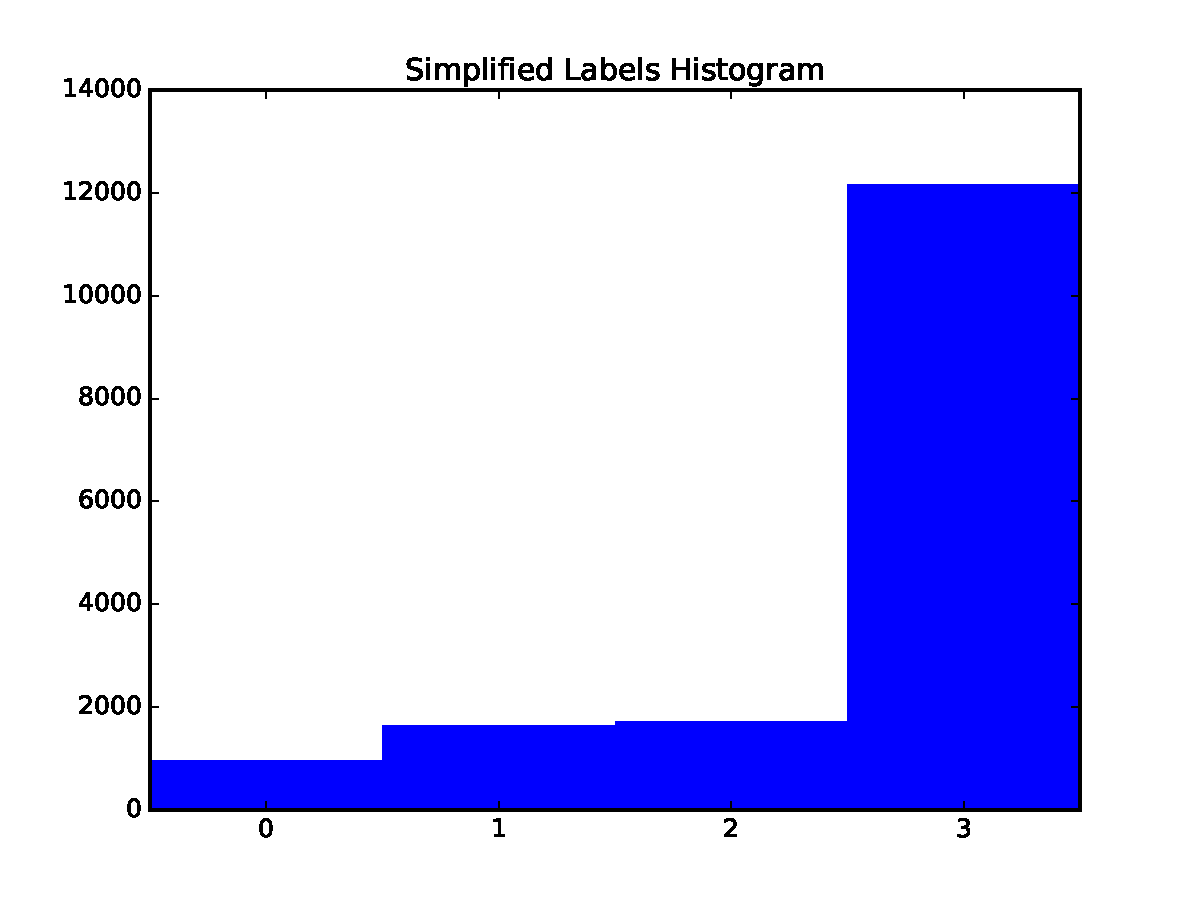
\includegraphics[width=\linewidth]{hist_simple_labels.pdf}
        \caption{Distribution of simplified labels in original dataset}
        \label{fig:singlelabeldistr}
    \end{minipage}
    \hfill
    \begin{minipage}{.49\linewidth}
        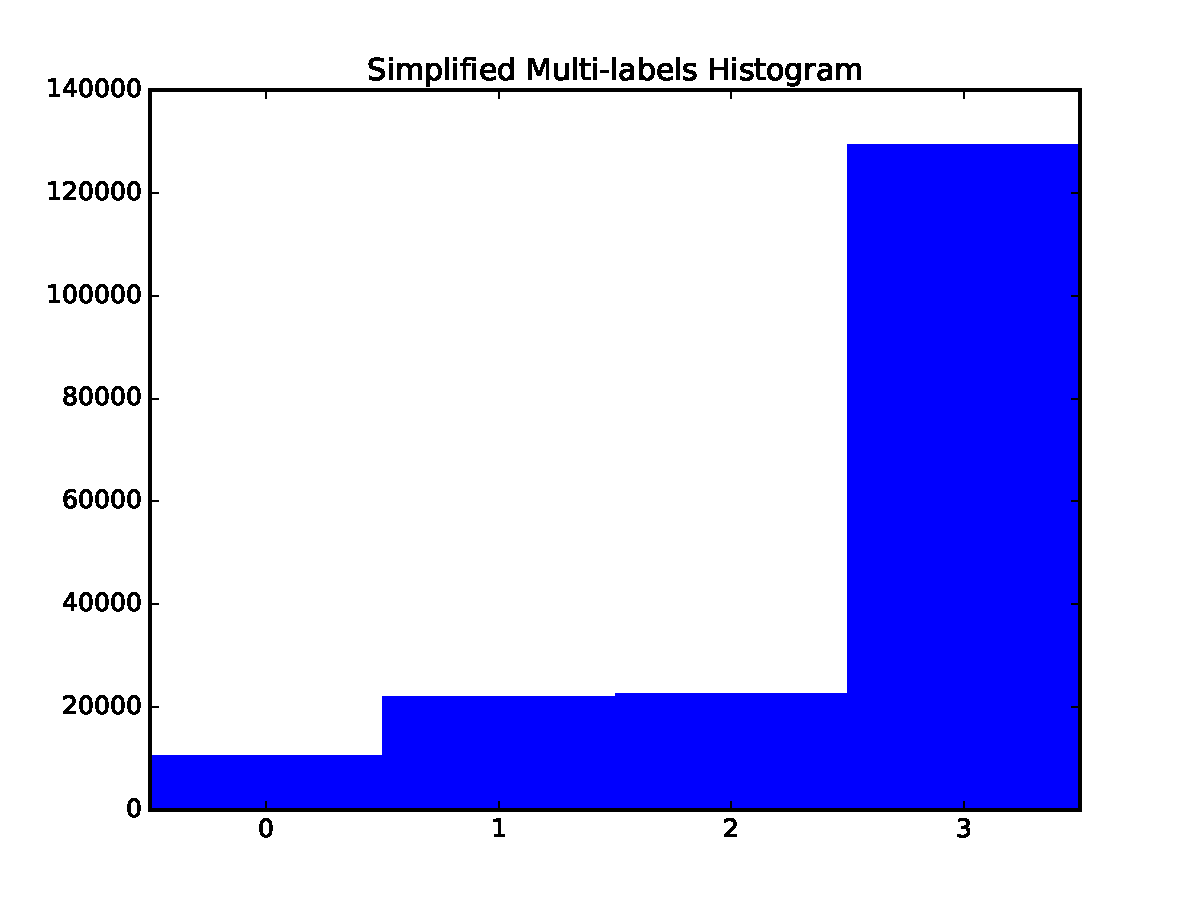
\includegraphics[width=\linewidth]{hist_simple_multi_labels.pdf}
        \caption{Distribution of simplified labels in multi-label outputs}
        \label{fig:multilabeldistr}
    \end{minipage}
\end{figure}

Note that from this point onwards, we will be working with the reduced feature set, in line with the aim of the paper to show the advantages of dirichlet multinomial regression when studies (environmental or otherwise) are limited to lower resolution data where strictly assigning only a single label to the features at a given data point is not representative of the otherwise rich information available.

\subsection{Coordinates as features}
Due to the abundant bathymetry data that was available in the form of depth, rugosity and aspect at each available data point, there was reason not to include the coordinates themselves in the feature space. Whilst it does make sense that in a natural environment, areas that were spatially near to one another would also have similar properties, this should not be relied upon, and other intrinsic properties should be the basis upon which predictions are made. Forming predictions on the full query dataset using a random forest supports this notion quite strongly - whilst 10-fold cross validation using the coordinates as features had a notably higher F-score of 0.61 compared to 0.40 without, the unnaturally straight split between the left and right segments over a 12km region suggests that the predictive map is flawed. Moreover, by including the coordinates as a training feature, an assertion is made about the direct relationship between a benthic location and the habitat class/es it contains, despite having other bathymetry information such as depth, aspect, etc. 

\todo{(argument/s here alone is/are weak. for simplified labels using coords is still much better by a similar (small) margin, do some reading to back this up properly)}

\begin{figure}[H]
    \begin{minipage}{.49\linewidth}
        \includegraphics[width=\linewidth]{full_predictions_randomforest.pdf}
        \caption{Full predictive map using Random Forests including coordinates as features}
        \label{fig:rf_w_coords_preds}
    \end{minipage}
    \hfill
    \begin{minipage}{.49\linewidth}
        \includegraphics[width=\linewidth]{full_predictions_randomforest_nocoords.pdf}
        \caption{Full predictive map using Random Forests excluding coordinates as features}
        \label{fig:rf_wo_coords_preds}
    \end{minipage}
\end{figure}

\subsection{Preprocessing and Feature Projection}
To maximise performance (in terms of minimising error/maximising the correctness metrics used) of the algorithms used across the experiments, a number of preprocessing steps were taken to ultimately improve the performance of the predictions made. The features in the data were first scaled, where each feature was centred to the mean with unit variance), then normalised over each future such that they had unit length \todo{(include plots of the diff approaches across DM/GP/others, ref plots)}. To further minimise bias and variance, the original feature set (which from this point onwards refers to all the non-coordinate features) was projected into higher dimensions, using combinations of features in higher degrees. \todo{(ref plots)}

\todo{(show plots)}

As evident from above, adding the square ($^2$) of each feature with a 1 regulariser \todo{(figure out what 1 column should be called)} yielded in performance that was negligibly lower ($\sim 1e-5$) than projection into full quadratic space, whilst requiring considerably fewer features - 19 for the former, vs. 55 for the latter. While this difference isn't significant for GPs \todo{(perhaps provide a time benchmark for this too)}, it has a significant effect on running time later on when using Markov Chain Monte Carlo (MCMC) to obtain draws of the weights of the Dirichlet Multinomial Regressor - when working with the simplified 4-label case, there are $19*4 =76 \text{ vs. } 55*4=220$ weights, i.e. dimensions to deal with, whereas the full 24-label case would involve $19*24=456$ and $55*24=1320$ weights respectively, which would result in a very significant increase in computing power needed for the MCMC chains to converge in the latter case, relatively speaking.
